
% Default to the notebook output style

    


% Inherit from the specified cell style.




    
\documentclass[11pt]{article}

    
    
    \usepackage[T1]{fontenc}
    % Nicer default font (+ math font) than Computer Modern for most use cases
    \usepackage{mathpazo}

    % Basic figure setup, for now with no caption control since it's done
    % automatically by Pandoc (which extracts ![](path) syntax from Markdown).
    \usepackage{graphicx}
    % We will generate all images so they have a width \maxwidth. This means
    % that they will get their normal width if they fit onto the page, but
    % are scaled down if they would overflow the margins.
    \makeatletter
    \def\maxwidth{\ifdim\Gin@nat@width>\linewidth\linewidth
    \else\Gin@nat@width\fi}
    \makeatother
    \let\Oldincludegraphics\includegraphics
    % Set max figure width to be 80% of text width, for now hardcoded.
    \renewcommand{\includegraphics}[1]{\Oldincludegraphics[width=.8\maxwidth]{#1}}
    % Ensure that by default, figures have no caption (until we provide a
    % proper Figure object with a Caption API and a way to capture that
    % in the conversion process - todo).
    \usepackage{caption}
    \DeclareCaptionLabelFormat{nolabel}{}
    \captionsetup{labelformat=nolabel}

    \usepackage{adjustbox} % Used to constrain images to a maximum size 
    \usepackage{xcolor} % Allow colors to be defined
    \usepackage{enumerate} % Needed for markdown enumerations to work
    \usepackage{geometry} % Used to adjust the document margins
    \usepackage{amsmath} % Equations
    \usepackage{amssymb} % Equations
    \usepackage{textcomp} % defines textquotesingle
    % Hack from http://tex.stackexchange.com/a/47451/13684:
    \AtBeginDocument{%
        \def\PYZsq{\textquotesingle}% Upright quotes in Pygmentized code
    }
    \usepackage{upquote} % Upright quotes for verbatim code
    \usepackage{eurosym} % defines \euro
    \usepackage[mathletters]{ucs} % Extended unicode (utf-8) support
    \usepackage[utf8x]{inputenc} % Allow utf-8 characters in the tex document
    \usepackage{fancyvrb} % verbatim replacement that allows latex
    \usepackage{grffile} % extends the file name processing of package graphics 
                         % to support a larger range 
    % The hyperref package gives us a pdf with properly built
    % internal navigation ('pdf bookmarks' for the table of contents,
    % internal cross-reference links, web links for URLs, etc.)
    \usepackage{hyperref}
    \usepackage{longtable} % longtable support required by pandoc >1.10
    \usepackage{booktabs}  % table support for pandoc > 1.12.2
    \usepackage[inline]{enumitem} % IRkernel/repr support (it uses the enumerate* environment)
    \usepackage[normalem]{ulem} % ulem is needed to support strikethroughs (\sout)
                                % normalem makes italics be italics, not underlines
    

    
    
    % Colors for the hyperref package
    \definecolor{urlcolor}{rgb}{0,.145,.698}
    \definecolor{linkcolor}{rgb}{.71,0.21,0.01}
    \definecolor{citecolor}{rgb}{.12,.54,.11}

    % ANSI colors
    \definecolor{ansi-black}{HTML}{3E424D}
    \definecolor{ansi-black-intense}{HTML}{282C36}
    \definecolor{ansi-red}{HTML}{E75C58}
    \definecolor{ansi-red-intense}{HTML}{B22B31}
    \definecolor{ansi-green}{HTML}{00A250}
    \definecolor{ansi-green-intense}{HTML}{007427}
    \definecolor{ansi-yellow}{HTML}{DDB62B}
    \definecolor{ansi-yellow-intense}{HTML}{B27D12}
    \definecolor{ansi-blue}{HTML}{208FFB}
    \definecolor{ansi-blue-intense}{HTML}{0065CA}
    \definecolor{ansi-magenta}{HTML}{D160C4}
    \definecolor{ansi-magenta-intense}{HTML}{A03196}
    \definecolor{ansi-cyan}{HTML}{60C6C8}
    \definecolor{ansi-cyan-intense}{HTML}{258F8F}
    \definecolor{ansi-white}{HTML}{C5C1B4}
    \definecolor{ansi-white-intense}{HTML}{A1A6B2}

    % commands and environments needed by pandoc snippets
    % extracted from the output of `pandoc -s`
    \providecommand{\tightlist}{%
      \setlength{\itemsep}{0pt}\setlength{\parskip}{0pt}}
    \DefineVerbatimEnvironment{Highlighting}{Verbatim}{commandchars=\\\{\}}
    % Add ',fontsize=\small' for more characters per line
    \newenvironment{Shaded}{}{}
    \newcommand{\KeywordTok}[1]{\textcolor[rgb]{0.00,0.44,0.13}{\textbf{{#1}}}}
    \newcommand{\DataTypeTok}[1]{\textcolor[rgb]{0.56,0.13,0.00}{{#1}}}
    \newcommand{\DecValTok}[1]{\textcolor[rgb]{0.25,0.63,0.44}{{#1}}}
    \newcommand{\BaseNTok}[1]{\textcolor[rgb]{0.25,0.63,0.44}{{#1}}}
    \newcommand{\FloatTok}[1]{\textcolor[rgb]{0.25,0.63,0.44}{{#1}}}
    \newcommand{\CharTok}[1]{\textcolor[rgb]{0.25,0.44,0.63}{{#1}}}
    \newcommand{\StringTok}[1]{\textcolor[rgb]{0.25,0.44,0.63}{{#1}}}
    \newcommand{\CommentTok}[1]{\textcolor[rgb]{0.38,0.63,0.69}{\textit{{#1}}}}
    \newcommand{\OtherTok}[1]{\textcolor[rgb]{0.00,0.44,0.13}{{#1}}}
    \newcommand{\AlertTok}[1]{\textcolor[rgb]{1.00,0.00,0.00}{\textbf{{#1}}}}
    \newcommand{\FunctionTok}[1]{\textcolor[rgb]{0.02,0.16,0.49}{{#1}}}
    \newcommand{\RegionMarkerTok}[1]{{#1}}
    \newcommand{\ErrorTok}[1]{\textcolor[rgb]{1.00,0.00,0.00}{\textbf{{#1}}}}
    \newcommand{\NormalTok}[1]{{#1}}
    
    % Additional commands for more recent versions of Pandoc
    \newcommand{\ConstantTok}[1]{\textcolor[rgb]{0.53,0.00,0.00}{{#1}}}
    \newcommand{\SpecialCharTok}[1]{\textcolor[rgb]{0.25,0.44,0.63}{{#1}}}
    \newcommand{\VerbatimStringTok}[1]{\textcolor[rgb]{0.25,0.44,0.63}{{#1}}}
    \newcommand{\SpecialStringTok}[1]{\textcolor[rgb]{0.73,0.40,0.53}{{#1}}}
    \newcommand{\ImportTok}[1]{{#1}}
    \newcommand{\DocumentationTok}[1]{\textcolor[rgb]{0.73,0.13,0.13}{\textit{{#1}}}}
    \newcommand{\AnnotationTok}[1]{\textcolor[rgb]{0.38,0.63,0.69}{\textbf{\textit{{#1}}}}}
    \newcommand{\CommentVarTok}[1]{\textcolor[rgb]{0.38,0.63,0.69}{\textbf{\textit{{#1}}}}}
    \newcommand{\VariableTok}[1]{\textcolor[rgb]{0.10,0.09,0.49}{{#1}}}
    \newcommand{\ControlFlowTok}[1]{\textcolor[rgb]{0.00,0.44,0.13}{\textbf{{#1}}}}
    \newcommand{\OperatorTok}[1]{\textcolor[rgb]{0.40,0.40,0.40}{{#1}}}
    \newcommand{\BuiltInTok}[1]{{#1}}
    \newcommand{\ExtensionTok}[1]{{#1}}
    \newcommand{\PreprocessorTok}[1]{\textcolor[rgb]{0.74,0.48,0.00}{{#1}}}
    \newcommand{\AttributeTok}[1]{\textcolor[rgb]{0.49,0.56,0.16}{{#1}}}
    \newcommand{\InformationTok}[1]{\textcolor[rgb]{0.38,0.63,0.69}{\textbf{\textit{{#1}}}}}
    \newcommand{\WarningTok}[1]{\textcolor[rgb]{0.38,0.63,0.69}{\textbf{\textit{{#1}}}}}
    
    
    % Define a nice break command that doesn't care if a line doesn't already
    % exist.
    \def\br{\hspace*{\fill} \\* }
    % Math Jax compatability definitions
    \def\gt{>}
    \def\lt{<}
    % Document parameters
    \title{Assignment 2}
    
    
    

    % Pygments definitions
    
\makeatletter
\def\PY@reset{\let\PY@it=\relax \let\PY@bf=\relax%
    \let\PY@ul=\relax \let\PY@tc=\relax%
    \let\PY@bc=\relax \let\PY@ff=\relax}
\def\PY@tok#1{\csname PY@tok@#1\endcsname}
\def\PY@toks#1+{\ifx\relax#1\empty\else%
    \PY@tok{#1}\expandafter\PY@toks\fi}
\def\PY@do#1{\PY@bc{\PY@tc{\PY@ul{%
    \PY@it{\PY@bf{\PY@ff{#1}}}}}}}
\def\PY#1#2{\PY@reset\PY@toks#1+\relax+\PY@do{#2}}

\expandafter\def\csname PY@tok@w\endcsname{\def\PY@tc##1{\textcolor[rgb]{0.73,0.73,0.73}{##1}}}
\expandafter\def\csname PY@tok@c\endcsname{\let\PY@it=\textit\def\PY@tc##1{\textcolor[rgb]{0.25,0.50,0.50}{##1}}}
\expandafter\def\csname PY@tok@cp\endcsname{\def\PY@tc##1{\textcolor[rgb]{0.74,0.48,0.00}{##1}}}
\expandafter\def\csname PY@tok@k\endcsname{\let\PY@bf=\textbf\def\PY@tc##1{\textcolor[rgb]{0.00,0.50,0.00}{##1}}}
\expandafter\def\csname PY@tok@kp\endcsname{\def\PY@tc##1{\textcolor[rgb]{0.00,0.50,0.00}{##1}}}
\expandafter\def\csname PY@tok@kt\endcsname{\def\PY@tc##1{\textcolor[rgb]{0.69,0.00,0.25}{##1}}}
\expandafter\def\csname PY@tok@o\endcsname{\def\PY@tc##1{\textcolor[rgb]{0.40,0.40,0.40}{##1}}}
\expandafter\def\csname PY@tok@ow\endcsname{\let\PY@bf=\textbf\def\PY@tc##1{\textcolor[rgb]{0.67,0.13,1.00}{##1}}}
\expandafter\def\csname PY@tok@nb\endcsname{\def\PY@tc##1{\textcolor[rgb]{0.00,0.50,0.00}{##1}}}
\expandafter\def\csname PY@tok@nf\endcsname{\def\PY@tc##1{\textcolor[rgb]{0.00,0.00,1.00}{##1}}}
\expandafter\def\csname PY@tok@nc\endcsname{\let\PY@bf=\textbf\def\PY@tc##1{\textcolor[rgb]{0.00,0.00,1.00}{##1}}}
\expandafter\def\csname PY@tok@nn\endcsname{\let\PY@bf=\textbf\def\PY@tc##1{\textcolor[rgb]{0.00,0.00,1.00}{##1}}}
\expandafter\def\csname PY@tok@ne\endcsname{\let\PY@bf=\textbf\def\PY@tc##1{\textcolor[rgb]{0.82,0.25,0.23}{##1}}}
\expandafter\def\csname PY@tok@nv\endcsname{\def\PY@tc##1{\textcolor[rgb]{0.10,0.09,0.49}{##1}}}
\expandafter\def\csname PY@tok@no\endcsname{\def\PY@tc##1{\textcolor[rgb]{0.53,0.00,0.00}{##1}}}
\expandafter\def\csname PY@tok@nl\endcsname{\def\PY@tc##1{\textcolor[rgb]{0.63,0.63,0.00}{##1}}}
\expandafter\def\csname PY@tok@ni\endcsname{\let\PY@bf=\textbf\def\PY@tc##1{\textcolor[rgb]{0.60,0.60,0.60}{##1}}}
\expandafter\def\csname PY@tok@na\endcsname{\def\PY@tc##1{\textcolor[rgb]{0.49,0.56,0.16}{##1}}}
\expandafter\def\csname PY@tok@nt\endcsname{\let\PY@bf=\textbf\def\PY@tc##1{\textcolor[rgb]{0.00,0.50,0.00}{##1}}}
\expandafter\def\csname PY@tok@nd\endcsname{\def\PY@tc##1{\textcolor[rgb]{0.67,0.13,1.00}{##1}}}
\expandafter\def\csname PY@tok@s\endcsname{\def\PY@tc##1{\textcolor[rgb]{0.73,0.13,0.13}{##1}}}
\expandafter\def\csname PY@tok@sd\endcsname{\let\PY@it=\textit\def\PY@tc##1{\textcolor[rgb]{0.73,0.13,0.13}{##1}}}
\expandafter\def\csname PY@tok@si\endcsname{\let\PY@bf=\textbf\def\PY@tc##1{\textcolor[rgb]{0.73,0.40,0.53}{##1}}}
\expandafter\def\csname PY@tok@se\endcsname{\let\PY@bf=\textbf\def\PY@tc##1{\textcolor[rgb]{0.73,0.40,0.13}{##1}}}
\expandafter\def\csname PY@tok@sr\endcsname{\def\PY@tc##1{\textcolor[rgb]{0.73,0.40,0.53}{##1}}}
\expandafter\def\csname PY@tok@ss\endcsname{\def\PY@tc##1{\textcolor[rgb]{0.10,0.09,0.49}{##1}}}
\expandafter\def\csname PY@tok@sx\endcsname{\def\PY@tc##1{\textcolor[rgb]{0.00,0.50,0.00}{##1}}}
\expandafter\def\csname PY@tok@m\endcsname{\def\PY@tc##1{\textcolor[rgb]{0.40,0.40,0.40}{##1}}}
\expandafter\def\csname PY@tok@gh\endcsname{\let\PY@bf=\textbf\def\PY@tc##1{\textcolor[rgb]{0.00,0.00,0.50}{##1}}}
\expandafter\def\csname PY@tok@gu\endcsname{\let\PY@bf=\textbf\def\PY@tc##1{\textcolor[rgb]{0.50,0.00,0.50}{##1}}}
\expandafter\def\csname PY@tok@gd\endcsname{\def\PY@tc##1{\textcolor[rgb]{0.63,0.00,0.00}{##1}}}
\expandafter\def\csname PY@tok@gi\endcsname{\def\PY@tc##1{\textcolor[rgb]{0.00,0.63,0.00}{##1}}}
\expandafter\def\csname PY@tok@gr\endcsname{\def\PY@tc##1{\textcolor[rgb]{1.00,0.00,0.00}{##1}}}
\expandafter\def\csname PY@tok@ge\endcsname{\let\PY@it=\textit}
\expandafter\def\csname PY@tok@gs\endcsname{\let\PY@bf=\textbf}
\expandafter\def\csname PY@tok@gp\endcsname{\let\PY@bf=\textbf\def\PY@tc##1{\textcolor[rgb]{0.00,0.00,0.50}{##1}}}
\expandafter\def\csname PY@tok@go\endcsname{\def\PY@tc##1{\textcolor[rgb]{0.53,0.53,0.53}{##1}}}
\expandafter\def\csname PY@tok@gt\endcsname{\def\PY@tc##1{\textcolor[rgb]{0.00,0.27,0.87}{##1}}}
\expandafter\def\csname PY@tok@err\endcsname{\def\PY@bc##1{\setlength{\fboxsep}{0pt}\fcolorbox[rgb]{1.00,0.00,0.00}{1,1,1}{\strut ##1}}}
\expandafter\def\csname PY@tok@kc\endcsname{\let\PY@bf=\textbf\def\PY@tc##1{\textcolor[rgb]{0.00,0.50,0.00}{##1}}}
\expandafter\def\csname PY@tok@kd\endcsname{\let\PY@bf=\textbf\def\PY@tc##1{\textcolor[rgb]{0.00,0.50,0.00}{##1}}}
\expandafter\def\csname PY@tok@kn\endcsname{\let\PY@bf=\textbf\def\PY@tc##1{\textcolor[rgb]{0.00,0.50,0.00}{##1}}}
\expandafter\def\csname PY@tok@kr\endcsname{\let\PY@bf=\textbf\def\PY@tc##1{\textcolor[rgb]{0.00,0.50,0.00}{##1}}}
\expandafter\def\csname PY@tok@bp\endcsname{\def\PY@tc##1{\textcolor[rgb]{0.00,0.50,0.00}{##1}}}
\expandafter\def\csname PY@tok@fm\endcsname{\def\PY@tc##1{\textcolor[rgb]{0.00,0.00,1.00}{##1}}}
\expandafter\def\csname PY@tok@vc\endcsname{\def\PY@tc##1{\textcolor[rgb]{0.10,0.09,0.49}{##1}}}
\expandafter\def\csname PY@tok@vg\endcsname{\def\PY@tc##1{\textcolor[rgb]{0.10,0.09,0.49}{##1}}}
\expandafter\def\csname PY@tok@vi\endcsname{\def\PY@tc##1{\textcolor[rgb]{0.10,0.09,0.49}{##1}}}
\expandafter\def\csname PY@tok@vm\endcsname{\def\PY@tc##1{\textcolor[rgb]{0.10,0.09,0.49}{##1}}}
\expandafter\def\csname PY@tok@sa\endcsname{\def\PY@tc##1{\textcolor[rgb]{0.73,0.13,0.13}{##1}}}
\expandafter\def\csname PY@tok@sb\endcsname{\def\PY@tc##1{\textcolor[rgb]{0.73,0.13,0.13}{##1}}}
\expandafter\def\csname PY@tok@sc\endcsname{\def\PY@tc##1{\textcolor[rgb]{0.73,0.13,0.13}{##1}}}
\expandafter\def\csname PY@tok@dl\endcsname{\def\PY@tc##1{\textcolor[rgb]{0.73,0.13,0.13}{##1}}}
\expandafter\def\csname PY@tok@s2\endcsname{\def\PY@tc##1{\textcolor[rgb]{0.73,0.13,0.13}{##1}}}
\expandafter\def\csname PY@tok@sh\endcsname{\def\PY@tc##1{\textcolor[rgb]{0.73,0.13,0.13}{##1}}}
\expandafter\def\csname PY@tok@s1\endcsname{\def\PY@tc##1{\textcolor[rgb]{0.73,0.13,0.13}{##1}}}
\expandafter\def\csname PY@tok@mb\endcsname{\def\PY@tc##1{\textcolor[rgb]{0.40,0.40,0.40}{##1}}}
\expandafter\def\csname PY@tok@mf\endcsname{\def\PY@tc##1{\textcolor[rgb]{0.40,0.40,0.40}{##1}}}
\expandafter\def\csname PY@tok@mh\endcsname{\def\PY@tc##1{\textcolor[rgb]{0.40,0.40,0.40}{##1}}}
\expandafter\def\csname PY@tok@mi\endcsname{\def\PY@tc##1{\textcolor[rgb]{0.40,0.40,0.40}{##1}}}
\expandafter\def\csname PY@tok@il\endcsname{\def\PY@tc##1{\textcolor[rgb]{0.40,0.40,0.40}{##1}}}
\expandafter\def\csname PY@tok@mo\endcsname{\def\PY@tc##1{\textcolor[rgb]{0.40,0.40,0.40}{##1}}}
\expandafter\def\csname PY@tok@ch\endcsname{\let\PY@it=\textit\def\PY@tc##1{\textcolor[rgb]{0.25,0.50,0.50}{##1}}}
\expandafter\def\csname PY@tok@cm\endcsname{\let\PY@it=\textit\def\PY@tc##1{\textcolor[rgb]{0.25,0.50,0.50}{##1}}}
\expandafter\def\csname PY@tok@cpf\endcsname{\let\PY@it=\textit\def\PY@tc##1{\textcolor[rgb]{0.25,0.50,0.50}{##1}}}
\expandafter\def\csname PY@tok@c1\endcsname{\let\PY@it=\textit\def\PY@tc##1{\textcolor[rgb]{0.25,0.50,0.50}{##1}}}
\expandafter\def\csname PY@tok@cs\endcsname{\let\PY@it=\textit\def\PY@tc##1{\textcolor[rgb]{0.25,0.50,0.50}{##1}}}

\def\PYZbs{\char`\\}
\def\PYZus{\char`\_}
\def\PYZob{\char`\{}
\def\PYZcb{\char`\}}
\def\PYZca{\char`\^}
\def\PYZam{\char`\&}
\def\PYZlt{\char`\<}
\def\PYZgt{\char`\>}
\def\PYZsh{\char`\#}
\def\PYZpc{\char`\%}
\def\PYZdl{\char`\$}
\def\PYZhy{\char`\-}
\def\PYZsq{\char`\'}
\def\PYZdq{\char`\"}
\def\PYZti{\char`\~}
% for compatibility with earlier versions
\def\PYZat{@}
\def\PYZlb{[}
\def\PYZrb{]}
\makeatother


    % Exact colors from NB
    \definecolor{incolor}{rgb}{0.0, 0.0, 0.5}
    \definecolor{outcolor}{rgb}{0.545, 0.0, 0.0}



    
    % Prevent overflowing lines due to hard-to-break entities
    \sloppy 
    % Setup hyperref package
    \hypersetup{
      breaklinks=true,  % so long urls are correctly broken across lines
      colorlinks=true,
      urlcolor=urlcolor,
      linkcolor=linkcolor,
      citecolor=citecolor,
      }
    % Slightly bigger margins than the latex defaults
    
    \geometry{verbose,tmargin=1in,bmargin=1in,lmargin=1in,rmargin=1in}
    
    

    \begin{document}
    
    
    \maketitle
    
    

    
%    \section{Assignment 2}\label{assignment-2}
\begin{center}
\textbf{COMP 4107 Fall 2017}

\textbf{Basim Ramadhan 100 901 646}

\textbf{Christian Abbott 100 863 049}
\end{center}

\begin{center}\rule{0.5\linewidth}{\linethickness}\end{center}

\textbf{NOTE: in our plots, the x-axis label should read "epoch"
instead of "fold number". In each training epoch, we are using the
entire training set using k-fold cross
validation.}\label{note-in-our-plots-the-x-axis-label-should-read-epoch-instead-of-fold-number.-in-each-training-epoch-we-are-using-the-entire-training-set-using-k-fold-cross-validation.}

\section{Running Our Code}\label{running-our-code}
    
    To train and test our network, simply run one of the following commands.
    To avoid running the full 300 epochs, use the second command. The
    program required that the MNIST dataset is available in a directory
    named mnist-data. We have included that directory with the data inside it in as part of our submission.
    
    \begin{Verbatim}[commandchars=\\\{\}]
    \PY{c+c1}{\PYZsh{} Run 300 epochs}
    \PY{n}{python3} \PY{n}{feedforward}\PY{o}{.}\PY{n}{py}
    \PY{c+c1}{\PYZsh{} Run X epochs}
    \PY{n}{python3} \PY{n}{feedforward}\PY{o}{.}\PY{n}{py} \PY{n}{X}
    \end{Verbatim}
    
\hspace{-16px}You will need to have numpy, scipy, and matplotlib installed.

    \section{Performing K-fold Cross
Correlation}\label{performing-k-fold-cross-correlation}

In our training process we used K-fold cross correlation to validate
the accuracy of our classifier, ensuring we don't have significant
generalization errors. It also helped us ensure we are not underfitting
or overfitting. The following code demonstrates that we used K-fold
cross correlation during training.

In each epoch, we use a different subset of training data to validate
our classifier's output. The MNIST training set contains 60000 elements.
Assuming we do 10-fold cross validation and we run 100 epochs: in the
first epoch, we use the first 6000 elements of the training set for
validation, and the remaining 54000 elements to train. In the second
epoch, we use the second subset of 6000 elements for validation, and the
remaining 54000 elements to train, and so on until we complete 100 epochs.
After we use the final 6000 subset of training elements for validation,
we roll back to using the first subset of 6000.

    \begin{Verbatim}[commandchars=\\\{\}]
{\color{incolor}In [{\color{incolor} }]:} \PY{n}{num\PYZus{}folds} \PY{o}{=} \PY{n+nb}{int}\PY{p}{(}\PY{n}{num\PYZus{}training\PYZus{}examples} \PY{o}{/} \PY{n}{net}\PY{o}{.}\PY{n}{batch\PYZus{}size}\PY{p}{)}
        \PY{n}{train\PYZus{}error} \PY{o}{=} \PY{p}{[}\PY{p}{]}
        \PY{n}{test\PYZus{}error} \PY{o}{=} \PY{p}{[}\PY{p}{]}
        \PY{n}{cv\PYZus{}error} \PY{o}{=} \PY{p}{[}\PY{p}{]}
        
        \PY{k}{for} \PY{n}{k} \PY{o+ow}{in} \PY{n+nb}{range}\PY{p}{(}\PY{n}{num\PYZus{}folds}\PY{p}{)}\PY{p}{:}
            \PY{c+c1}{\PYZsh{} Deep copy the training set because we want to manipulate it}
            \PY{n}{x} \PY{o}{=} \PY{n}{np}\PY{o}{.}\PY{n}{copy}\PY{p}{(}\PY{n}{train\PYZus{}x}\PY{p}{)}
            \PY{n}{y} \PY{o}{=} \PY{n}{np}\PY{o}{.}\PY{n}{copy}\PY{p}{(}\PY{n}{train\PYZus{}y}\PY{p}{)}\PY{o}{.}\PY{n}{reshape}\PY{p}{(}\PY{l+m+mi}{1}\PY{p}{,} \PY{l+m+mi}{60000}\PY{p}{)}
            \PY{n}{y\PYZus{}oh} \PY{o}{=} \PY{n}{np}\PY{o}{.}\PY{n}{copy}\PY{p}{(}\PY{n}{train\PYZus{}y\PYZus{}onehot}\PY{p}{)}
        
            \PY{c+c1}{\PYZsh{} Indices of the cross\PYZhy{}validation (test) examples}
            \PY{n}{cv\PYZus{}start} \PY{o}{=} \PY{n}{net}\PY{o}{.}\PY{n}{batch\PYZus{}size} \PY{o}{*} \PY{n}{k}
            \PY{n}{cv\PYZus{}end} \PY{o}{=} \PY{n}{net}\PY{o}{.}\PY{n}{batch\PYZus{}size} \PY{o}{*} \PY{p}{(}\PY{n}{k} \PY{o}{+} \PY{l+m+mi}{1}\PY{p}{)}
        
            \PY{c+c1}{\PYZsh{} Get the cross\PYZhy{}validation (test) examples}
            \PY{n}{cv\PYZus{}columns} \PY{o}{=} \PY{p}{[}\PY{n}{x} \PY{k}{for} \PY{n}{x} \PY{o+ow}{in} \PY{n+nb}{range}\PY{p}{(}\PY{n}{cv\PYZus{}start}\PY{p}{,} \PY{n}{cv\PYZus{}end}\PY{p}{)}\PY{p}{]}
            \PY{n}{cv\PYZus{}x} \PY{o}{=} \PY{n}{x}\PY{p}{[}\PY{p}{:}\PY{p}{,} \PY{n}{cv\PYZus{}columns}\PY{p}{]}
            \PY{n}{cv\PYZus{}y} \PY{o}{=} \PY{n}{y}\PY{p}{[}\PY{p}{:}\PY{p}{,} \PY{n}{cv\PYZus{}columns}\PY{p}{]}
            \PY{n}{cv\PYZus{}y\PYZus{}oh} \PY{o}{=} \PY{n}{y\PYZus{}oh}\PY{p}{[}\PY{p}{:}\PY{p}{,} \PY{n}{cv\PYZus{}columns}\PY{p}{]}
        
            \PY{c+c1}{\PYZsh{} Remove cross\PYZhy{}validation (test) examples from the training set}
            \PY{n}{x} \PY{o}{=} \PY{n}{np}\PY{o}{.}\PY{n}{delete}\PY{p}{(}\PY{n}{x}\PY{p}{,} \PY{n}{cv\PYZus{}columns}\PY{p}{,} \PY{l+m+mi}{1}\PY{p}{)}
            \PY{n}{y} \PY{o}{=} \PY{n}{np}\PY{o}{.}\PY{n}{delete}\PY{p}{(}\PY{n}{y}\PY{p}{,} \PY{n}{cv\PYZus{}columns}\PY{p}{,} \PY{l+m+mi}{1}\PY{p}{)}
            \PY{n}{y\PYZus{}oh} \PY{o}{=} \PY{n}{np}\PY{o}{.}\PY{n}{delete}\PY{p}{(}\PY{n}{y\PYZus{}oh}\PY{p}{,} \PY{n}{cv\PYZus{}columns}\PY{p}{,} \PY{l+m+mi}{1}\PY{p}{)}
        
            \PY{c+c1}{\PYZsh{} Shuffle the training examples for better results}
            \PY{n}{x}\PY{p}{,} \PY{n}{y}\PY{p}{,} \PY{n}{y\PYZus{}oh} \PY{o}{=} \PY{n}{net}\PY{o}{.}\PY{n}{shuffle\PYZus{}training\PYZus{}set}\PY{p}{(}\PY{n}{x}\PY{p}{,} \PY{n}{y}\PY{p}{,} \PY{n}{y\PYZus{}oh}\PY{p}{)}
        
            \PY{n}{training\PYZus{}batches} \PY{o}{=} \PY{n+nb}{filter}\PY{p}{(}\PY{k}{lambda} \PY{n}{fold}\PY{p}{:} \PY{n}{fold} \PY{o}{!=} \PY{n}{k}\PY{p}{,} \PY{n+nb}{range}\PY{p}{(}\PY{n}{num\PYZus{}folds}\PY{o}{\PYZhy{}}\PY{l+m+mi}{1}\PY{p}{)}\PY{p}{)}
            \PY{k}{for} \PY{n}{i} \PY{o+ow}{in} \PY{n}{training\PYZus{}batches}\PY{p}{:}
                \PY{n}{batch\PYZus{}start} \PY{o}{=} \PY{n}{net}\PY{o}{.}\PY{n}{batch\PYZus{}size} \PY{o}{*} \PY{n}{i}
                \PY{n}{batch\PYZus{}end} \PY{o}{=} \PY{n}{net}\PY{o}{.}\PY{n}{batch\PYZus{}size} \PY{o}{*} \PY{p}{(}\PY{n}{i} \PY{o}{+} \PY{l+m+mi}{1}\PY{p}{)}
        
                \PY{n}{x\PYZus{}batch} \PY{o}{=} \PY{n}{np}\PY{o}{.}\PY{n}{array}\PY{p}{(}\PY{p}{[}\PY{n}{row}\PY{p}{[}\PY{n}{batch\PYZus{}start}\PY{p}{:}\PY{n}{batch\PYZus{}end}\PY{p}{]} \PY{k}{for} \PY{n}{row} \PY{o+ow}{in} \PY{n}{x}\PY{p}{]}\PY{p}{)}
                \PY{n}{y\PYZus{}batch} \PY{o}{=} \PY{n}{np}\PY{o}{.}\PY{n}{array}\PY{p}{(}\PY{p}{[}\PY{n}{row}\PY{p}{[}\PY{n}{batch\PYZus{}start}\PY{p}{:}\PY{n}{batch\PYZus{}end}\PY{p}{]} \PY{k}{for} \PY{n}{row} \PY{o+ow}{in} \PY{n}{y\PYZus{}oh}\PY{p}{]}\PY{p}{)}
        
                \PY{n}{a}\PY{p}{,} \PY{n}{o} \PY{o}{=} \PY{n}{net}\PY{o}{.}\PY{n}{\PYZus{}propagate}\PY{p}{(}\PY{n}{x\PYZus{}batch}\PY{p}{)}
                \PY{n}{d} \PY{o}{=} \PY{n}{net}\PY{o}{.}\PY{n}{\PYZus{}backpropagate}\PY{p}{(}\PY{n}{y\PYZus{}batch}\PY{p}{)}
                \PY{n}{net}\PY{o}{.}\PY{n}{\PYZus{}adjust\PYZus{}weights}\PY{p}{(}\PY{p}{)}
                \PY{n}{net}\PY{o}{.}\PY{n}{\PYZus{}adjust\PYZus{}biases}\PY{p}{(}\PY{p}{)}
\end{Verbatim}

\pagebreak

\section{Using Weight Decay for Regularization}\label{using-weight-decay-for-regularization}

We added a hyperparameter called weight\_decay which we used to
regularize our weights. The following code demonstrates that we used
weight decay when updating our network's weights.

    \begin{Verbatim}[commandchars=\\\{\}]
\PY{k}{for} \PY{n}{weight}\PY{p}{,} \PY{n}{delta}\PY{p}{,} \PY{n}{activation} \PY{o+ow}{in} \PY{n+nb}{zip}\PY{p}{(}\PY{n+nb+bp}{self}\PY{o}{.}\PY{n}{\PYZus{}w}\PY{p}{,} \PY{n+nb+bp}{self}\PY{o}{.}\PY{n}{\PYZus{}d}\PY{p}{,} \PY{n+nb+bp}{self}\PY{o}{.}\PY{n}{\PYZus{}a}\PY{p}{)}\PY{p}{:}
    \PY{n}{regularization} \PY{o}{=} \PY{p}{(}\PY{n}{learn\PYZus{}rate} \PY{o}{*} \PY{n+nb+bp}{self}\PY{o}{.}\PY{n}{weight\PYZus{}decay}\PY{p}{)} \PY{o}{*} \PY{n}{weight}
    \PY{n}{new\PYZus{}w} \PY{o}{=} \PY{n}{weight} \PY{o}{\PYZhy{}} \PY{n}{learn\PYZus{}rate} \PY{o}{*} \PY{n}{np}\PY{o}{.}\PY{n}{dot}\PY{p}{(}\PY{n}{delta}\PY{p}{,} \PY{n}{activation}\PY{o}{.}\PY{n}{T}\PY{p}{)} \PY{o}{\PYZhy{}} \PY{n}{regularization}
    \PY{n}{new\PYZus{}weights}\PY{o}{.}\PY{n}{append}\PY{p}{(}\PY{n}{new\PYZus{}w}\PY{p}{)}
\end{Verbatim}


    The following code shows how we used the weight decay hyperparameter
again when updating our network's biases:

    \begin{Verbatim}[commandchars=\\\{\}]
\PY{k}{for} \PY{n}{bias}\PY{p}{,} \PY{n}{delta} \PY{o+ow}{in} \PY{n+nb}{zip}\PY{p}{(}\PY{n+nb+bp}{self}\PY{o}{.}\PY{n}{\PYZus{}b}\PY{p}{,} \PY{n+nb+bp}{self}\PY{o}{.}\PY{n}{\PYZus{}d}\PY{p}{)}\PY{p}{:}
    \PY{n}{regularization} \PY{o}{=} \PY{p}{(}\PY{n}{learn\PYZus{}rate} \PY{o}{*} \PY{n+nb+bp}{self}\PY{o}{.}\PY{n}{weight\PYZus{}decay}\PY{p}{)} \PY{o}{*} \PY{n}{bias}
    \PY{n}{new\PYZus{}b} \PY{o}{=} \PY{n}{bias} \PY{o}{\PYZhy{}} \PY{n}{learn\PYZus{}rate} \PY{o}{*} \PY{p}{(}\PY{n}{np}\PY{o}{.}\PY{n}{sum}\PY{p}{(}\PY{n}{delta}\PY{p}{,} \PY{n}{axis}\PY{o}{=}\PY{l+m+mi}{1}\PY{p}{)}\PY{p}{)}\PY{o}{.}\PY{n}{reshape}\PY{p}{(}\PY{n}{bias}\PY{o}{.}\PY{n}{shape}\PY{p}{)} \PY{o}{\PYZhy{}} \PY{n}{regularization}
    \PY{n}{new\PYZus{}biases}\PY{o}{.}\PY{n}{append}\PY{p}{(}\PY{n}{new\PYZus{}b}\PY{p}{)}
\end{Verbatim}

The use of weight decay helped reduce the generalization error by ensuring large weights do not get out of control.


\pagebreak

\section{Investigating Performance for Different Numbers of Hidden
Layers}\label{investigating-performance-for-different-numbers-of-hidden-layers}

For each of the following experiements, we used:
\begin{itemize}
	\item Learning Rate: \textbf{0.005}
	\item Weight Decay: \textbf{0.2}
	\item Number of folds: \textbf{100}
	\item Epochs: \textbf{100}
\end{itemize}

\subsection{Zero Hidden Layers}\label{zero-hidden-layers}

\begin{figure}[htbp]
\centering
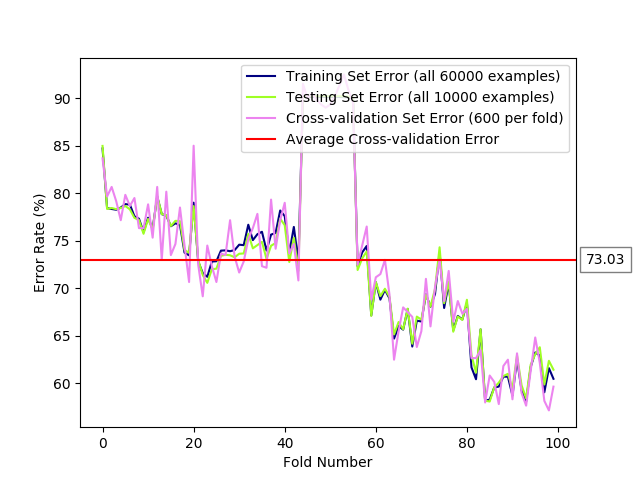
\includegraphics{plots/ff-numlayers-0.png}
\end{figure}

\paragraph{Architecture}\label{architecture}

\begin{itemize}
\tightlist
\item
  Input layer: 784
\item
  Output Layer: 10
\end{itemize}

\paragraph{Result}\label{result}

Average cross validation error: \textbf{73.03\%}

First, we tried training a network with no hidden layers. The poor
performance indicates that the 10-label MNIST classification problem warrants \textbf{at least} 
one hidden layer for accurate classification.

\pagebreak

\subsection{One Hidden Layer}\label{one-hidden-layer}

\begin{figure}[htbp]
\centering
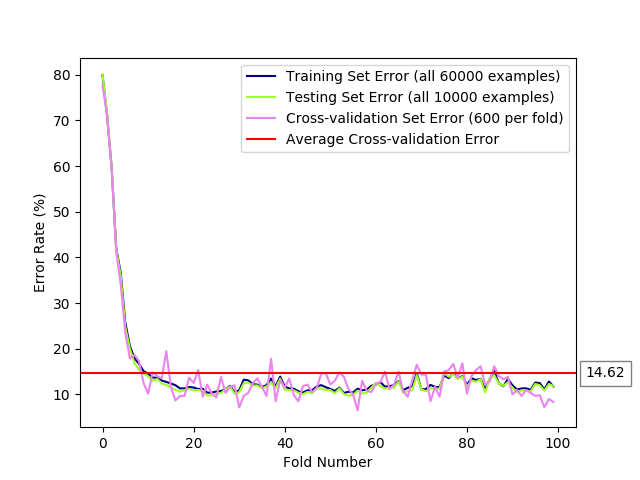
\includegraphics{plots/ff-numlayers-60.png}
\end{figure}

\paragraph{Architecture}\label{architecture-1}

\begin{itemize}
\tightlist
\item
  Input layer: 784
\item
  Hidden Layer: 60
\item
  Output Layer: 10
\end{itemize}

\paragraph{Result}\label{result}

Average 100-fold cross validation error: \textbf{14.62\%}

It looks like the classifier works reasonably well with only one
hidden layer. Let's keep adding layers to see how it affects accuracy.

\pagebreak

\subsection{Two Hidden Layers}\label{two-hidden-layers}

\begin{figure}[htbp]
\centering
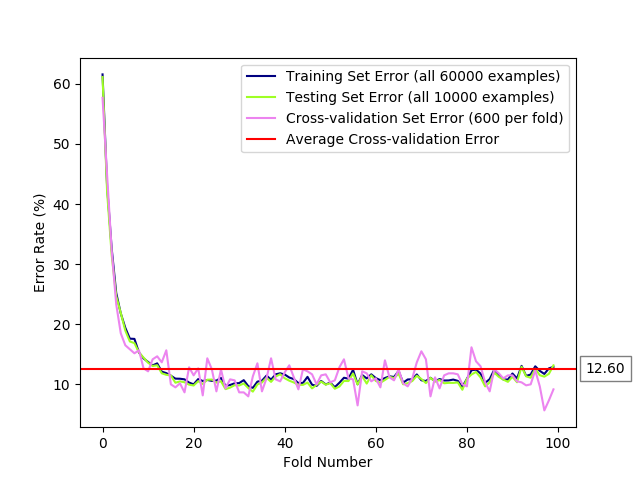
\includegraphics{plots/ff-numlayers-60-30.png}
\end{figure}

\paragraph{Architecture}\label{architecture-2}

\begin{itemize}
\tightlist
\item
  Input layer: 784
\item
  Hidden Layer 1: 60
\item
  Hidden Layer 2: 30
\item
  Output Layer: 10
\end{itemize}

\paragraph{Result}\label{result-1}

Average 100-fold cross validation error: \textbf{12.60\%}

Adding a second layer helps a little bit without slowing down training
very much.

\pagebreak

\subsection{Three Hidden Layers}\label{three-hidden-layers}

\begin{figure}[htbp]
\centering
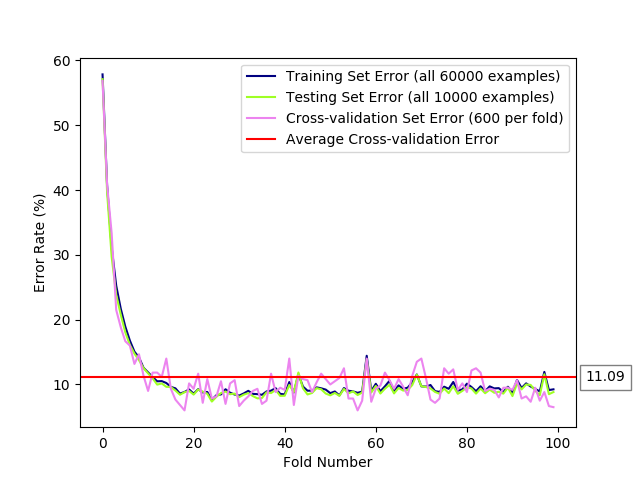
\includegraphics{plots/ff-numlayers-120-60-30.png}
\end{figure}

\paragraph{Architecture}\label{architecture-3}

\begin{itemize}
\tightlist
\item
  Input layer: 784
\item
  Hidden Layer 1: 120
\item
  Hidden Layer 2: 60
\item
  Hidden Layer 3: 30
\item
  Output Layer: 10
\end{itemize}

\paragraph{Result}\label{result-2}

Average 100-fold cross validation error: \textbf{11.09\%}

The third layer didn't help as much as adding the second layer did.
Perhaps a third is unnecesary.

\pagebreak

\subsubsection{Four Hidden Layers}\label{four-hidden-layers}

\begin{figure}[htbp]
\centering
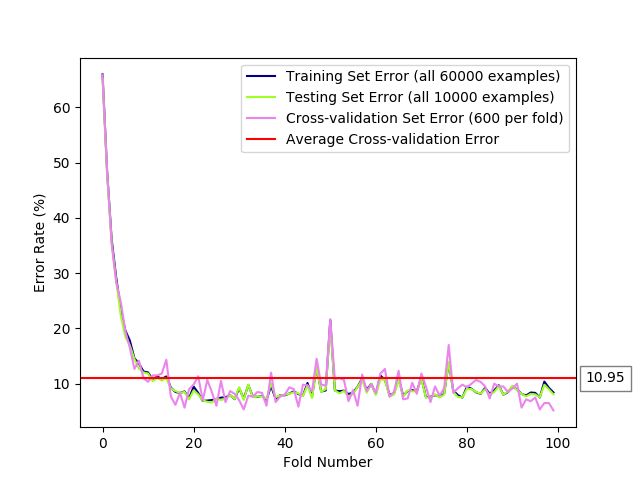
\includegraphics{plots/ff-numlayers-240-120-60-30.png}
\caption{ff-numlayers-240-120-60-30.png}
\end{figure}

\paragraph{Architecture}\label{architecture-4}

\begin{itemize}
\tightlist
\item
  Input layer: 784
\item
  Hidden Layer 1: 240
\item
  Hidden Layer 2: 120
\item
  Hidden Layer 3: 60
\item
  Hidden Layer 4: 30
\item
  Output Layer: 10
\end{itemize}

\paragraph{Result}\label{result-3}

Average 100-fold cross validation error: \textbf{10.95\%}

Again, the additional layer helped a little bit, but with each new
layer, training time becomes longer. We haven't seen much improvement
since having one hidden layer, so it looks like we must improve
our classifier's accuracy through other means.

\pagebreak

\subsection{Conclusions}\label{conclusions}

\begin{figure}[htbp]
\centering
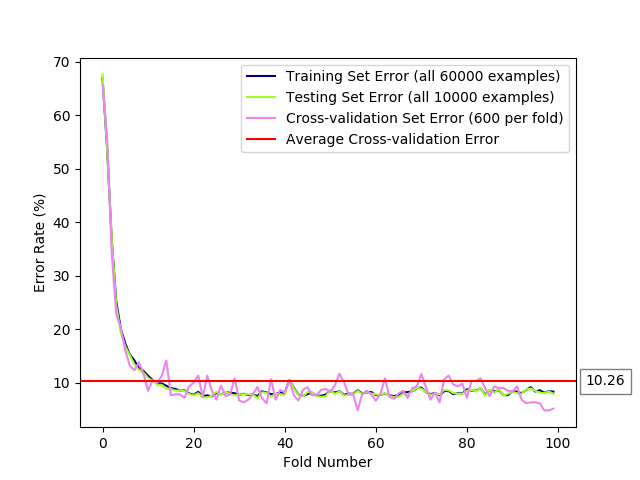
\includegraphics{plots/ff-numlayers-160-60-conclusion.png}
\caption{ff-numlayers-160-60-conclusion.png}
\end{figure}

\paragraph{Architecture}\label{architecture-5}

\begin{itemize}
\tightlist
\item
  Input layer: 784
\item
  Hidden Layer 1: 160
\item
  Hidden Layer 2: 60
\item
  Output Layer: 10
\end{itemize}

\paragraph{Result}\label{result-4}

100-fold cross validation error: \textbf{10.26\%}

After some experimentation, we settled on two hidden layers. It provided
a good balance between accuracy and training speed. Now we'll try
experimenting with the sizes of those two hidden layers to improve the
accuracy of the classifier.

\pagebreak

    \section{Investigating Performance for Different Sizes of Hidden
Layers}\label{investigating-performance-for-different-sizes-of-hidden-layers}

\subsection{Small Layers}\label{small-layers}

\begin{figure}[htbp]
\centering
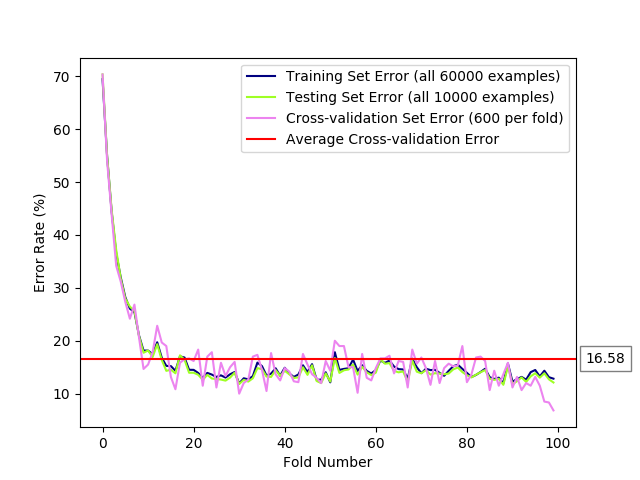
\includegraphics{plots/ff-layersize-30-15.png}
\end{figure}

\paragraph{Architecture}\label{architecture}

\begin{itemize}
\tightlist
\item
  Input layer: 784
\item
  Hidden Layer 1: 30
\item
  Hidden Layer 2: 15
\item
  Output Layer: 10
\end{itemize}

\paragraph{Result}\label{result}

Average 100-fold cross validation error: \textbf{16.58\%}

Making the layers very small doesn't give an awful classifier, but we
can easily improve this.

\pagebreak

\subsection{Medium Layers}\label{medium-layers}

\begin{figure}[htbp]
\centering
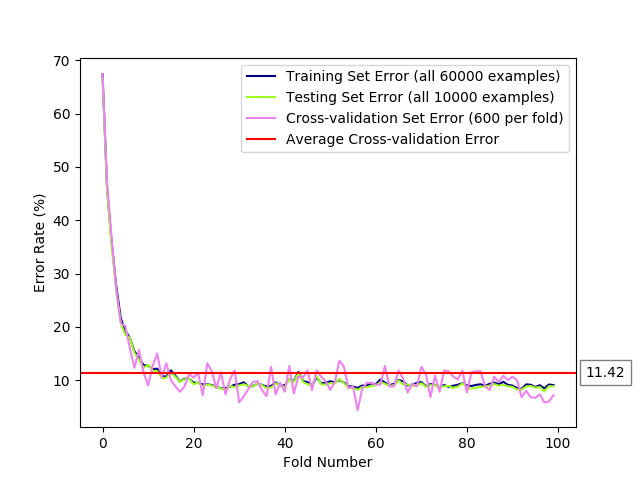
\includegraphics{plots/ff-layersize-100-50.png}
\end{figure}

\paragraph{Architecture}\label{architecture-1}

\begin{itemize}
\tightlist
\item
  Input layer: 784
\item
  Hidden Layer 1: 100
\item
  Hidden Layer 2: 50
\item
  Output Layer: 10
\end{itemize}

\paragraph{Result}\label{result-1}

Average 100-fold cross validation error: \textbf{11.42\%}

Making the layer bigger improved the accuracy of the classifier.

\pagebreak

\subsection{Large Layers}\label{large-layers}

\begin{figure}[htbp]
\centering
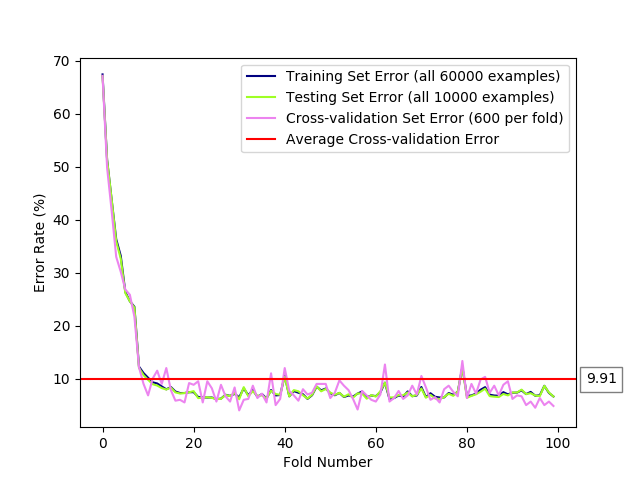
\includegraphics{plots/ff-layersize-300-100.png}
\end{figure}

\paragraph{Architecture}\label{architecture-2}

\begin{itemize}
\tightlist
\item
  Input layer: 784
\item
  Hidden Layer 1: 300
\item
  Hidden Layer 2: 100
\item
  Output Layer: 10
\end{itemize}

\paragraph{Result}\label{result-2}

Average 100-fold cross validation error: \textbf{9.91\%}

Making them even bigger helped even more.
\pagebreak

\subsection{Very Large Layers}\label{very-large-layers}

\begin{figure}[htbp]
\centering
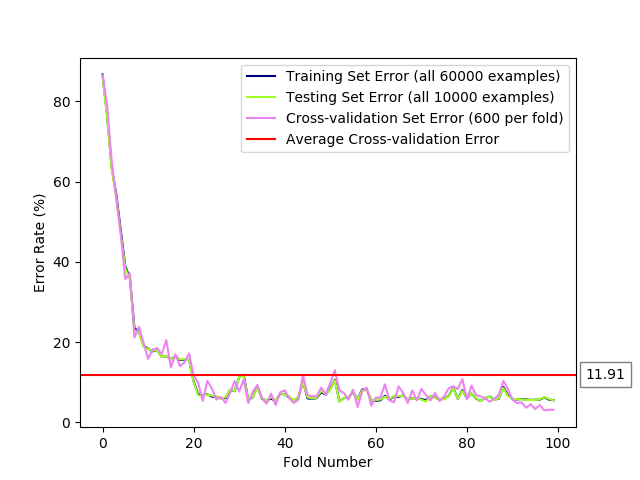
\includegraphics{plots/ff-layersize-500-200.png}
\end{figure}

\paragraph{Architecture}\label{architecture-3}

\begin{itemize}
\tightlist
\item
  Input layer: 784
\item
  Hidden Layer 1: 500
\item
  Hidden Layer 2: 200
\item
  Output Layer: 10
\end{itemize}

\paragraph{Result}\label{result-3}

Average 100-fold cross validation error: \textbf{11.91\%}

Making them too big has done the reverse. Let's make the layers smaller
and try to find a good ratio between the two layers.

\pagebreak

\subsection{Larger Same Size Layers}\label{larger-same-size-layers}

\begin{figure}[htbp]
\centering
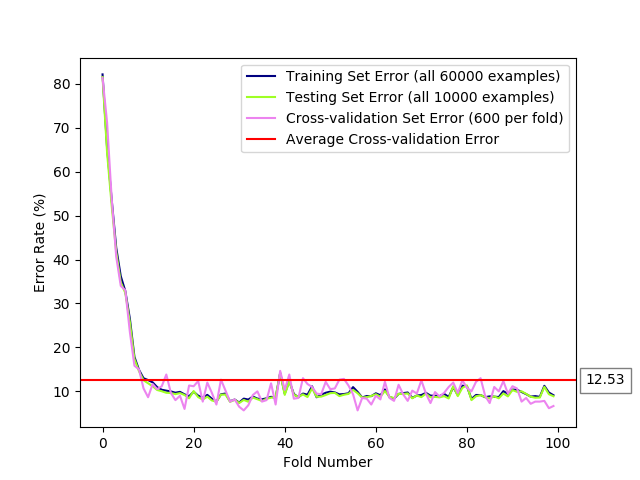
\includegraphics{plots/ff-layersize-128-128.png}
\end{figure}

\paragraph{Architecture}\label{architecture-4}

\begin{itemize}
\tightlist
\item
  Input layer: 784
\item
  Hidden Layer 1: 128
\item
  Hidden Layer 2: 128
\item
  Output Layer: 10
\end{itemize}

\paragraph{Result}\label{result-4}

Average 100-fold cross validation error: \textbf{12.54\%}

We tried using the same size for both hidden layer, but it didn't
improve accuracy. Perhaps making both of them smaller would help.

\pagebreak

\subsection{Smaller Same Size Layers}\label{smaller-same-size-layers}

\begin{figure}[htbp]
\centering
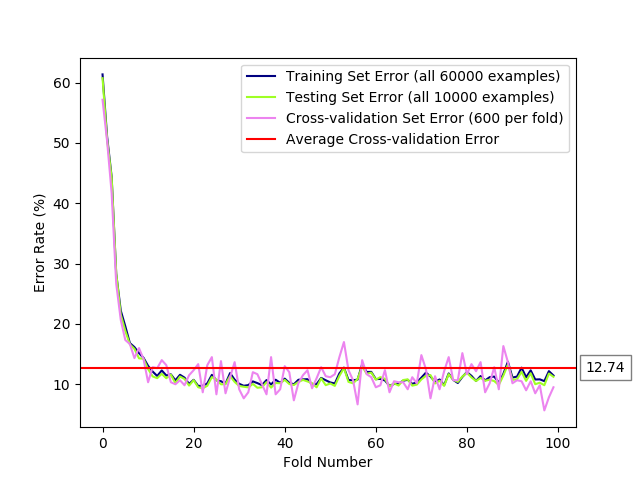
\includegraphics{plots/ff-layersize-64-64.png}
\caption{ff-layersize-64-64.png}
\end{figure}

\paragraph{Architecture:}\label{architecture-5}

\begin{itemize}
\tightlist
\item
  Input layer: 784
\item
  Hidden Layer 1: 64
\item
  Hidden Layer 2: 64
\item
  Output Layer: 10
\end{itemize}

\paragraph{Result}\label{result-5}

Average 100-fold cross validation error: \textbf{12.74\%}

We got a very similar result to using 128 for both hidden layers.
Perhaps a wide difference between hidden layers would help.

\pagebreak

\subsection{Layers With Wide Size
Difference}\label{layers-with-wide-size-difference}

\begin{figure}[htbp]
\centering
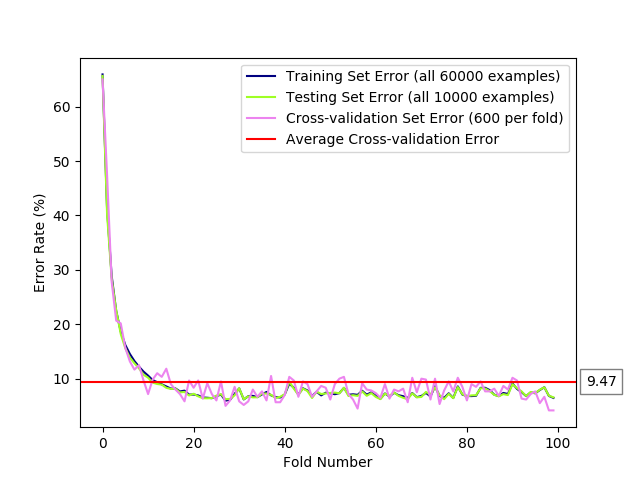
\includegraphics{plots/ff-layersize-300-40.png}
\caption{ff-layersize-300-40.png}
\end{figure}

\paragraph{Architecture}\label{architecture-6}

\begin{itemize}
\tightlist
\item
  Input layer: 784
\item
  Hidden Layer 1: 300
\item
  Hidden Layer 2: 40
\item
  Output Layer: 10
\end{itemize}

\paragraph{Result}\label{result-6}

100-fold cross validation error: \textbf{9.47\%}

It looks like a wide difference between the two layers helps the
classifier perform better, but not better than we've perviously seen.

\subsection{Conclusions}\label{conclusions}

We learned a few things here:
\begin{itemize}
	\item if the final hidden layer is too big,
accuracy goes down
	\item layers should not be too small
	\item layers should not be too big
	\item layers should not be the same size
	\item layers should have sizeable size differences between them
\end{itemize}

\pagebreak

    \section{Final Results + Statistical
Analysis}\label{final-results-our-best-performance-statistical-analysis}

\subsection{Our Best Performance}

In this run, we had the following error rates:
\begin{itemize}
	\item error when testing with the 10,000 element test dataset: \textbf{4.18\%}
	\item average cross-validation error over 300 folds: \textbf{6.65\%}
	\item average cross-validation error over final 30 folds: \textbf{2.67\%}
\end{itemize} 


\hspace{-16px}We used the following hyperparameters to achieve this:
\begin{itemize}
	\item MLP Architecture: \textbf{784, 160, 60, 10}
	\item Learning rate: \textbf{0.001}
	\item Weight Decay:	\textbf{0.2}
	\item Batch Size: \textbf{200}
	\item Epochs: \textbf{300}
\end{itemize}


\begin{figure}[htbp]
\centering
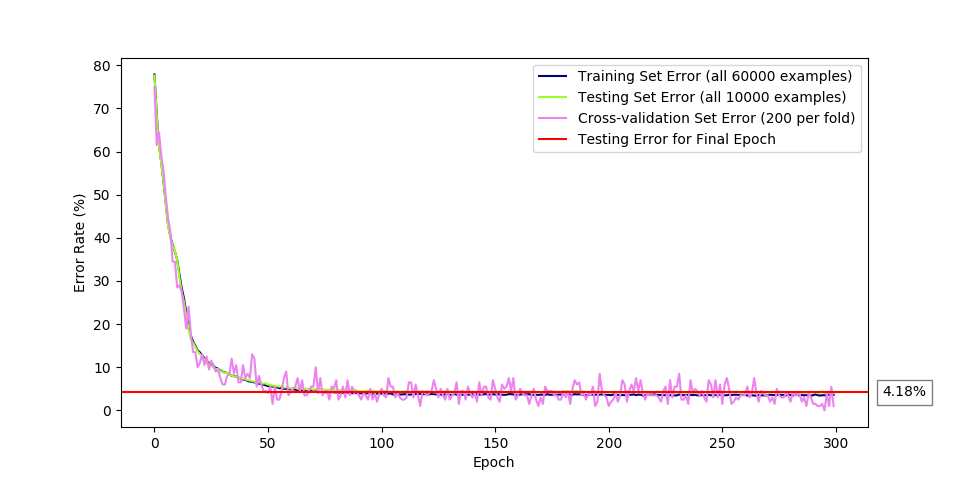
\includegraphics{plots/ff-bestest-performance-wide.png}
\end{figure}

We will use this result in the following section for statistical analysis.

\subsection{Mean Classification
Accuracy}\label{mean-classification-accuracy}

\subsubsection{For the mean classification error rate using the 10000
element test
set}\label{for-the-mean-classification-error-rate-using-the-10000-element-test-set}

We computed a \textbf{95\%} confidence interval for the test error of
the classifier after the final epoch. This value is the error rate when
using the \textbf{10,000 element testing set}. We used the following
code to compute the confidence interval. The code is part of our
submitted program; it runs after every time training is complete and
prints out the interval.

    \begin{Verbatim}[commandchars=\\\{\}]
\PY{n}{confidence} \PY{o}{=} \PY{l+m+mf}{0.95}
\PY{n}{samples} \PY{o}{=} \PY{n}{test\PYZus{}error}\PY{p}{[}\PY{o}{\PYZhy{}}\PY{n+nb}{int}\PY{p}{(}\PY{n}{epochs}\PY{o}{/}\PY{l+m+mi}{10}\PY{p}{)}\PY{p}{:}\PY{o}{\PYZhy{}}\PY{l+m+mi}{1}\PY{p}{]}
\PY{n}{mean} \PY{o}{=} \PY{n}{np}\PY{o}{.}\PY{n}{mean}\PY{p}{(}\PY{n}{samples}\PY{p}{)}
\PY{n}{sigma} \PY{o}{=} \PY{n}{np}\PY{o}{.}\PY{n}{std}\PY{p}{(}\PY{n}{samples}\PY{p}{)}
\PY{n}{interval} \PY{o}{=} \PY{n}{scipy.stats}\PY{o}{.}\PY{n}{norm}\PY{o}{.}\PY{n}{interval}\PY{p}{(}\PY{n}{confidence}\PY{p}{,} \PY{n}{loc}\PY{o}{=}\PY{n}{mean}\PY{p}{,} \PY{n}{scale}\PY{o}{=}\PY{n}{sigma}\PY{p}{)}
\end{Verbatim}


    Let \(X\) be a \textbf{random variable} representing the test error rate
of the classifier. We used the test error rate for the a portion of
epochs' test error rates---when the classifier has
converged---as samples to construct the \textbf{probability
distribution} for X. We did this to avoid the misleading values at the
first few epochs. This does not damage our results; it simply makes the
interval slightly larger. Considering the probability distribution, we
are \textbf{95\% confident} that the mean lies within the interval
\textbf{(3.99\%, 4.40\%)}.

\subsubsection{For the mean cross-validation error rate over 300
epochs}\label{for-the-mean-cross-validation-error-rate-over-300-folds}

Using the \textbf{same code} and \textbf{same approach} as the
subsection above, we computed the \textbf{95\%} confidence interval for
the mean cross-validation error over 300 epochs. We are 95\% confident
that the mean lies in the interval \textbf{(-12.08\%, 25.38\%)}

\subsubsection{For the mean cross-validation error rate over the final 30
epochs}\label{for-the-mean-cross-validation-error-rate-over-the-final-30-folds}

Since the above interval considers the values from the first few epochs,
we will use values from after the weights have converged. Using the
\textbf{same code} and \textbf{same approach} as the subsection above,
we computed the \textbf{95\%} confidence interval for the mean
cross-validation error over 30 epochs. We are 95\% confident that the
mean lies in the interval \textbf{(3.30\%, 5.30\%)}



\section{References}\label{references}

The work we provided in our submission is our own.

We referred to the following sources for simple matters like tweaking
hyperparameters and choosing layer sizes. The professor stated in the
forums that this is allowed:
https://culearn.carleton.ca/moodle/mod/forum/discuss.php?d=296418

\begin{itemize}
\tightlist
\item
  https://stats.stackexchange.com/questions/29130/difference-between-neural-net-weight-decay-and-learning-rate
\item
  https://github.com/andrewdyates/Radial-Basis-Function-Neural-Network
\item
  https://florianmuellerklein.github.io/nn/
\item
  https://github.com/FlorianMuellerklein/Machine-Learning/blob/master/MultiLayerPerceptron.py
\item
  https://github.com/hdmetor/NeuralNetwork
\item
  https://machinelearningmastery.com/report-classifier-performance-confidence-intervals/
\item
  https://stackoverflow.com/questions/28242593/correct-way-to-obtain-confidence-interval-with-scipy
\item
  https://machinelearningmastery.com/implement-backpropagation-algorithm-scratch-python/
\end{itemize}


    % Add a bibliography block to the postdoc
    
    
    
    \end{document}
